\section*{lecture 1 (04.04.2016)}
\subsection*{Introduction}

\begin{itemize}
 \item supervised learning: learn relaionships between variables
 \item unsupervised learning: learn some structure of measured variables
\end{itemize}

Dependend variables are measured at independant variables (covariates). Variables are measured on some \textbf{scale}:

\begin{itemize}
 \item nominal (gender, color)
 \item ordinal (ranking of soccerteams)
 \item interval (temperature in degree celsius)
 \item rational (temperature in kelvin, weight, height), has meaningful zero in comparison to interval
\end{itemize}

$\Rightarrow$ quotients make sense on ratio scale; quotiens of differences make sense on interval scale\\
metric scale: interval- and ratio scale  \\

\subsection*{problems in machine learning}:
\begin{enumerate}[1.]
 \item \textbf{regression}: one dependent variable on \textcolor{red}{metric scale}\\
 one or more independent variables on \textcolor{red}{metric scale}
 \item \textbf{variance analysis}: one dependent variable on \textcolor{red}{metric scale}\\
 one or more independent variables on \textcolor{red}{nominal scale}
 \item \textbf{classification}: one dependent variable on \textcolor{red}{nominal scale}\\
 one or more independent variables on \textcolor{red}{metric scale}
 \item \textbf{contingency analysis}: one dependent variable on \textcolor{red}{nominal scale}\\
 one or more independent variables on \textcolor{red}{nominal scale}
 \item \textbf{scaling problems}: independent variables on \textcolor{red}{arbitrary scale} but measurements on ordinal scale\\
 dependent variables on \textcolor{red}{metric scale}
\end{enumerate}

\subsection*{linear regression}
data/measurements: $(x^{(1)}, y^{(1)}), \dots , (x^{(n)}, y^{(n)})$ \\\\
$x^{(i)}$ independent/covariates $\in \mathbb{R}^n$ ($n$ - variables)\\
$y^{(i)}$ dependent/variates $\in \mathbb{R}^n$\\
$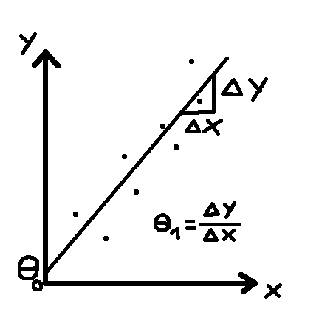
\includegraphics{graphs/plot.eps} \\
plot suggests a linear dependence between $x$ and $y$ \\
$y = \Theta_1 x + \Theta_0$\\\\
in the multivate case: $y = \Theta_0 + \Theta_1 X_1 + \dots + \Theta_n X_n$\\
$= \Theta^T X, X = (1, X_1, \dots ,X_n ) \in \mathbb{R}^{n+1}$\\\\

problem: estimate the parameter vector $\Theta in \mathbb{R}^{n+1}$ from the measurements $(x^{(1)}, y^{(1)}), \dots , (x^{(n)}, y^{(n)})$\\
loss function: $\textcolor{red}{L(\Theta)} = \frac{1}{2} \Sigma^m_{i=1} (\Theta^T X^{(i)} - y^{(i)})^2$\\
\textcolor{red}{model loss $\hat{=}$ loss for parameter vector $\Theta$}\\\\
goal: choose $\Theta \in \mathbb{R}^{n+1}$ that minimizes the loss function\\
reformulation:\\\\
data matrix:
\[ X =\left( \begin{array}{ccc}
x^{(1)^T} \\
\vdots \\
x^{(n)^T} \end{array} \right) \in \mathbb{R}^{m \times (n+1)}\]
response vector:

\[ Y =\left( \begin{array}{ccc}
y^{(1)} \\
\vdots \\
y^{(n)} \end{array} \right) \in \mathbb{R}^n\]
parameter vector:

\[ \Theta =\left( \begin{array}{ccc}
\Theta_0 \\
\vdots \\
\Theta_n \end{array} \right) \in \mathbb{R}^{n+1}\]
loss function in vectorized form:
\[L(\Theta) = \frac{1}{2} \Sigma^m_{i=1} (\Theta^T * X^{(i)} - Y^{(i)})^2 = \frac{1}{2} \lVert \textcolor{red}{X * \Theta} - \textcolor{blue}{Y} \lVert^2_2\]

\begin{center}
( \textcolor{red}{vector of predictions}$\quad\quad\quad$ \textcolor{blue}{vector of observation response} )
\end{center}
\[ = \frac{1}{2} (X * \Theta -Y)^T * (X * \Theta - Y)\]
\begin{center}
(definition of the euclidian norm)
\end{center}
\[ = \frac{1}{2} (\Theta^T X^T \times \Theta - \textcolor{red}{\Theta^T X^T Y - Y^T X*\Theta} + Y^T Y)\]
\begin{center}
= $-2 \Theta^T X^T Y$ since the dot product is symmetric ($X^T Y = Y^T X$)
\end{center}
\[= \frac{1}{2} \Theta^T X^T X \Theta - \Theta^T X^T Y + \frac{1}{2} Y^T Y\]
remember from calculus: A neccessary condition for an optimum of the (loss-) function is that the gradient vanishes.\\

$\bigtriangledown_{\Theta} L(\Theta) \stackrel{!}{=} 0 \quad\quad\quad\quad\quad\quad\quad\quad\quad  t(x) = \frac{1}{2}x^2+ax+b$\\
$\bigtriangledown_{\Theta} L(\Theta) = X^T X \Theta * X^T Y \stackrel{!}{=} 0  \quad\quad\quad \bigtriangledown_x t(x) = x+a$\\\\
here we have used that $X^T X$ is symmetric\\\\
$\Rightarrow X^T X \Theta = X^T Y \quad\quad\quad\quad\quad t(\Theta) = \Theta^T X \Theta$\\
$\Rightarrow  \Theta = (X^T X)^{-1} X^T Y \quad\quad\quad\quad\quad \bigtriangledown_{\Theta} t(\Theta) = (X+X^T)\Theta$\\
privided that $(X^T X)^{-1}$ exists\\\\
$\textcolor{red}{(X^T X)_{ij}} = X^{(i)^T}X^{(j)}$\\
\textcolor{red}{operation matrix}\\
dot product of i-th dataa point and j-th data point\\\\
hence, the last square solution of the linear regression problem is $\Theta = (X^T X)^{-1} X^T Y$\\\\
more robust solution:\\\\
$\Theta = (X^T X + \gamma \mathds{1})^{-1} X^T Y, \quad\quad \gamma > 0$ regularization parameter\\\\
ridge regression solution is not only more robust numerically, but also statistically (it is not so sensitive to small measurement errors in $X$).\\\\
Natural question: which loss function gives us the ridge regression solution?\\\\
answer: $\quad\quad L_{ridge} (\Theta)= \textcolor{red}{\frac{1}{2} \lVert X * \Theta - Y \lVert_2^2} + \textcolor{blue}{\gamma \lVert \Theta \lVert_2^2}$
\begin{center}
\textcolor{red}{loss term} \space\space \textcolor{blue}{reularisation term}
\end{center}
probabilistic interpretation of least squares
\[ Y = \textcolor{red}{\Theta^T * X} + \textcolor{blue}{\epsilon} \]
\begin{center}
\textcolor{red}{deterministic part} \space\space \textcolor{blue}{random/noise part}
\end{center}
model of the noise: gaussian noise \space\space $p(\epsilon)= \frac{1}{\sqrt{2\pi}\sigma} \exp (- \frac{\epsilon^2}{2 \sigma^2}) \quad$ (probability density function)\\
$P[a \leq \epsilon \leq b] = \int_a^b p(\epsilon)\quad d\epsilon$\\\\
$Y$ is a function of the random noise term $\epsilon$ als a random variable. The probability density function of $Y$ is:
\[ p(Y) = \frac{1}{\sqrt{2 \pi}\sigma} \exp(- \frac{\lVert Y - \Theta^T X \lVert^2_2}{2 \sigma^2})\]
